% !TeX root = ..\main.tex
% Chapter 3

\chapter{系统设计与实现}




本章主要介绍本系统的设计与实现,包括系统的整体架构、各个模块的功能和实现方法。

\section{系统架构概述}
本系统包含图像分析、古诗生成、古诗评价和古诗优化四个模块,基于Python语言开发,使用百度智能云提供的API接口来调用模型,整体架构如图~\ref{fig:system_architecture}所示。

% TODO 架构图重画,加入更多模型细节

\begin{figure}[h]
    \centering
    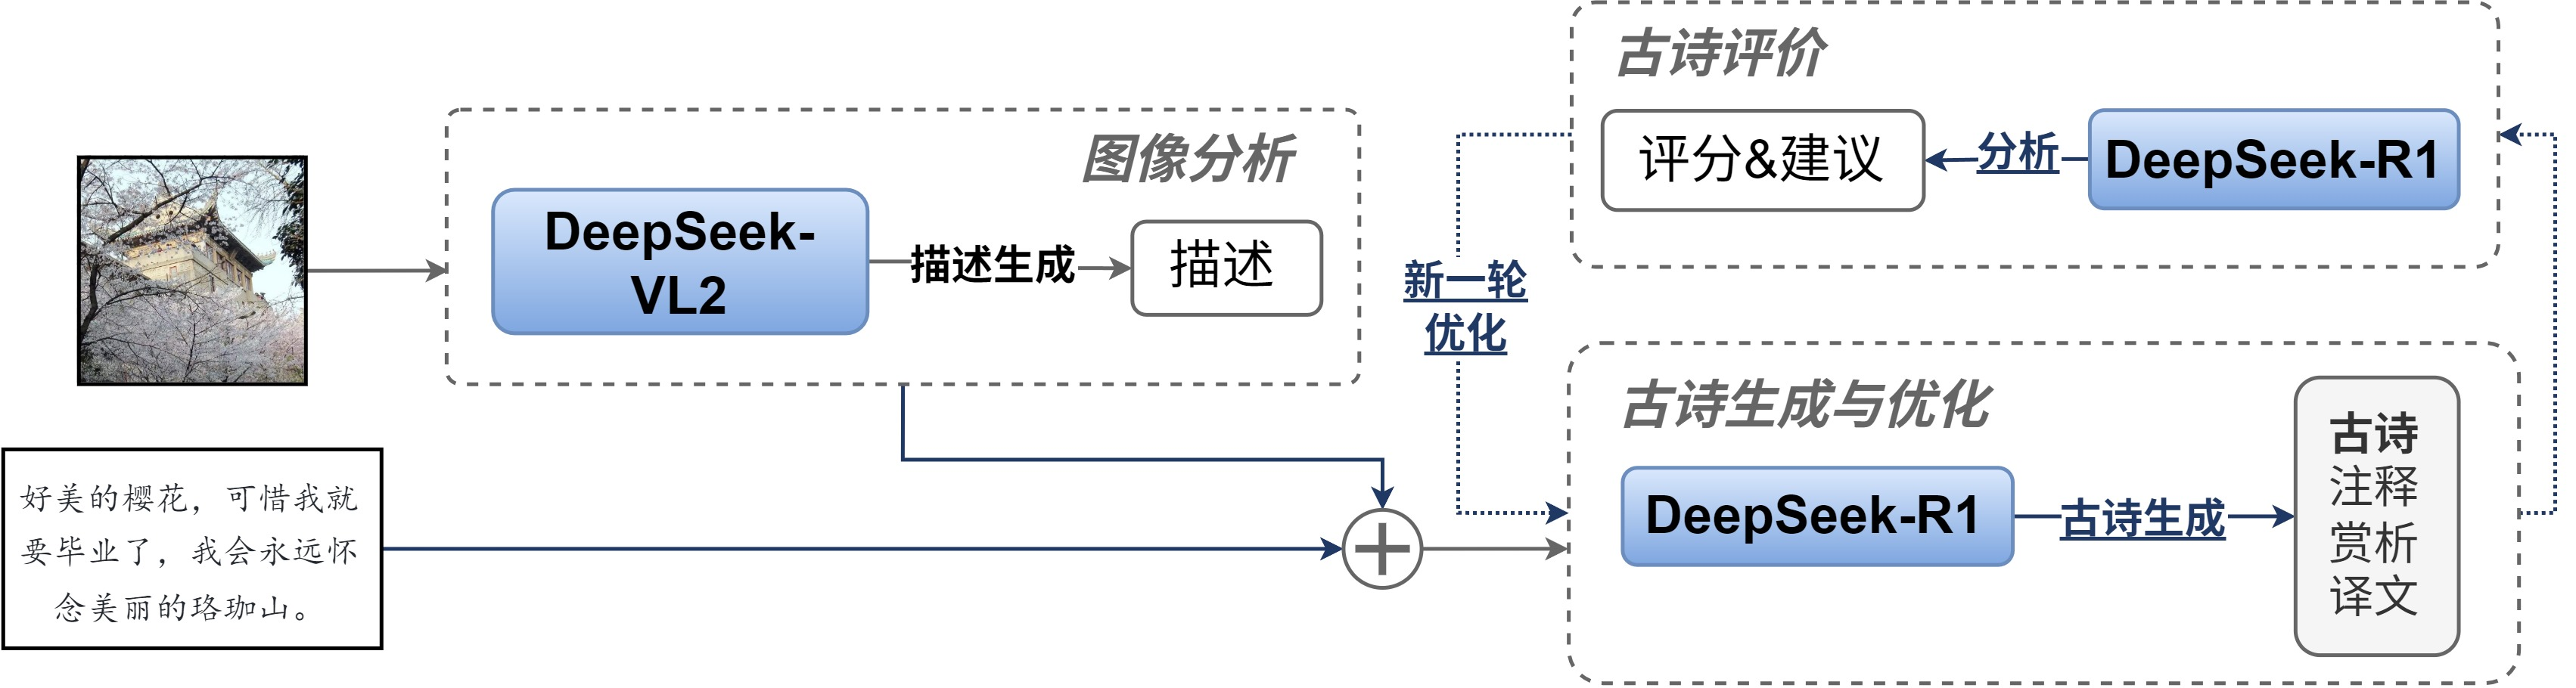
\includegraphics[width=1\textwidth]
    {figures/系统架构.jpg}\\
    \caption{系统架构}
    \label{fig:system_architecture}
  \end{figure}

\section{图像分析} \label{sec:image_analysis}

在先前的方案中,图像分析使用的是英文模型CLIP和MiniGPT-4,分别关注图像中的关键物体和整体描述,并最后交由ERNIE-4.0模型总结为中文描述。尽管生成的描述较精确、但无法捕捉有助于古诗创作的中国文化联想素材与情感色彩。举例而言,对图~\ref{fig:example_input}中的图像输入,先前的工作流输出结果如下%图~\ref{fig:previous_image_output}

\begin{figure}[ht]
  \centering
  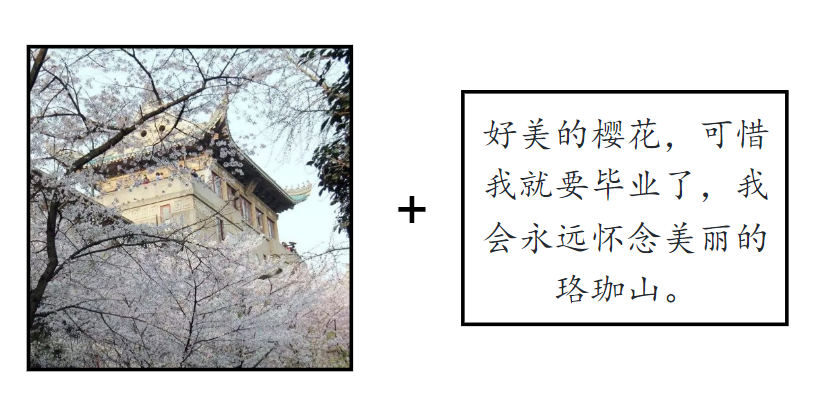
\includegraphics[width=0.65\textwidth]
  {figures/示例输入.png}\\
  \caption{示例输入}
  \label{fig:example_input} % 添加标签
\end{figure}

{\kaishu 
\textbf{CLIP:} Xinyang, Yunfu, Zhoukou, Blossom, Pagoda, Teahouse\par
\textbf{MiniGPT4:} The image shows \underline{a large, ornate building} with \underline{a tall, pointed roof} and \underline{a large, open balcony} on the second floor. The building is surrounded by a large, flowering cherry tree, which is in full bloom and covered in pink blossoms. There are several people standing on the sidewalk in front of the building, looking up at the cherry tree. The sky is clear and blue, with a few clouds in the distance. The building appears to be made of stone or brick, with intricate carvings and decorations on the facade. There are several other buildings in the background, some of which are also covered in blooming cherry trees. The overall scene is one of beauty and serenity. \par
\textbf{ERNIE-4.0:} 图中展示了一座装饰繁复的\underline{大型建筑},其拥有\underline{高耸的尖顶}和二楼宽敞的\underline{开放式阳台}。建筑被一棵盛开的樱花树环绕,满树繁花,粉白交错。建筑前的人行道上,数人驻足,仰头欣赏樱花的美丽。晴空万里,远处的几朵云彩点缀在蓝天之中。这座看似由砖石砌成的建筑,立面雕刻精美,装饰繁复。背景中还有其他几座建筑,其中一些同样被盛开的樱花所簇拥。整幅画面洋溢着美丽与宁静的气息。
}

可以发现,虽然最终的文字准确描述了画面内容,但依旧无法生成符合古诗创作需求的文化意象:
\begin{itemize}
  \item CLIP误读文化符号:CLIP输出的“Teahouse”(茶室)与“Pagoda”(塔)形成文化错位,这一点源于CLIP的训练数据分布偏差——在西方语料库中,“pagoda”常与日本茶道场景关联,而中文语境下塔与茶室并无必然联系,况且画面中的建筑并不是塔。更严重的是,模型甚至输出了“Xinyang”(信阳)、“Yunfu”(云浮)等意义难明的拼音,暴露了其对中文地理文化符号的认知缺失。
  \item MiniGPT4直译式描述:MiniGPT-4虽然能识别“樱花树”“尖顶建筑”等元素,但描述方式太平实直白。例如将中式建筑的“飞檐”简单说成“pointed roof”(尖顶),而将樱花描述为“pink blossoms”(粉色花朵),这种直译式描述丢失了文化内涵。
  % \item 情感表达机械化:ERNIE-4.0总结时,常使用“美丽与宁静”这类泛泛之词。例如面对繁花盛开的画面,模型无法像古诗那样通过“感时花溅泪”表达深层情感。它只是简单判断画面“美丽”,却无法捕捉中国人“乐景衬哀情”的复杂心境。就像用“开心”描述《红楼梦》中黛玉葬花的场景,完全体会不到其中的哀愁。
\end{itemize}

于是,当CLIP和MiniGPT4的输出交由ERNIE-4.0来总结时,最后的结果也难免停留在缺失文化内涵的直译文本,“只识其形,不知其意”,无法进一步提供与中国传统文化要素的关联。
% **根本问题在于**:现有模型像“外语翻译器”而非“文化解码器”。它们能识别物体(如樱花、建筑),但无法理解这些物体背后的文化意义(如樱花象征生命短暂,飞檐体现古代工艺)。当需要生成古诗时,这种“只识其形,不知其意”的缺陷,导致文字缺乏打动人心的文化力量。

因此,本文尝试直接使用中文语境下的图像大模型替代之前的多模型组合方案,一步到位地为图像生成兼顾关键物体识别、整体场景信息和情感色彩的描述。使用相同的图像输入,结合简单的提示词对不同的中文图像模型进行测试。提示词见图~\ref{fig:prompt_image_analysis}

\begin{figure}[ht]
  \begin{tcolorbox}[
      colback=white, % 背景透明
      colframe=black, 
      boxrule=1pt,        % 设置边框宽度
      arc=0mm             % 取消圆角
      ]
      \kaishu 请描述这张图片,注意要明确提及图像中的物体,描述清楚物体的色彩、大小、相对位置等基本信息,并兼顾整体的情感色彩,确保读者能够根据描述在心里构建出一个清晰的画面。请确保使用中文,不超过7句话,并使用一个段落完成。
      % \caption{图像分析提示词}
  \end{tcolorbox}
  \caption{提示词(图像分析)}
  \label{fig:prompt_image_analysis} % 添加标签
\end{figure}


初步测试发现,在较小的参数规模时,DeepSeek-VL2\upcite{wuDeepSeekVL2MixtureofExpertsVisionLanguage2024}(4.5B)的表现较好于Qwen2.5-VL-3B。二者的输出如下:%,但二者都不如参数规模更大的Qwen2.5-VL-32B的输出那样更具美感。

{\kaishu 
\textbf{DeepSeek-VL2:} 这张图片展示了一座传统中式建筑,其屋顶装饰着精美的\underline{绿色琉璃瓦},显得庄重典雅。\underline{建筑主体为浅黄色},四周有栏杆围绕,似乎有游客站在阳台上欣赏风景。前景是繁茂的樱花树,\underline{粉白色的花朵}覆盖了大部分画面,营造出浪漫而宁静的氛围。天空清澈,与花朵的柔和色彩形成鲜明对比,增添了画面的层次感。整幅画面让人感受到春天生机勃勃的气息,同时也透露出一种悠闲和诗意的情感。\par
\textbf{Qwen2.5-VL-3B:} 这张图片展示了一座传统的中国建筑,可能是寺庙或宫殿。建筑的屋顶是典型的翘角设计,\underline{颜色为黄色和绿色}。建筑周围有许多盛开的樱花树,花朵呈现出粉红色,与建筑的色彩形成了美丽的对比。树木的枝叶繁茂,覆盖了大部分画面。在建筑的阳台上,可以看到一些人在欣赏风景。整体氛围宁静而美丽,给人一种春天的感觉。\par
%\textbf{Qwen2.5-VL-32B:} 这张图片展示了一座古色古香的建筑,背景是盛开的樱花树,营造出一种宁静而浪漫的氛围。建筑的屋顶是典型的中式风格,飞檐翘角,屋檐下有精美的雕刻装饰,显得庄重而典雅。建筑的外墙以浅色为主,窗户和门框则呈现出红色,增添了古典的韵味。建筑的顶部有一些游客在平台上观赏风景,增添了画面的生动感。前景中,盛开的樱花树枝繁叶茂,粉色的花朵密密麻麻地覆盖在枝头,与建筑的古朴色调形成了鲜明的对比。樱花树的枝干粗壮,交错纵横,显得生机勃勃。整体画面充满了春天的气息,给人一种宁静、祥和且略带诗意的感觉。
}
可以看到,前者的输出描述了更具象的色彩意象,而后者仍只提供视觉要素的平面罗列。以色彩为例,前者的输出包含有“绿色琉璃瓦”、“浅黄建筑”、“粉白樱花”等精确的色彩描述,而后者只模糊地提及“黄色和绿色”。而在空间层次上,前者通过“前景樱花-中景建筑-远景天空”的立体构图清晰地描述出了图像中的立体信息,而后者却丢失了这份空间关系的描述。

因此,本文使用DeepSeek-VL2作为图像描述模型,一步到位为用户输入的图像生成充分体现空间信息、具有中式美感的描述文本,为进一步的古诗创作提供充分的视觉感官描述。

在调用百度智能云的API接口时,需要提供提示词和图像的URL地址,而不是直接将图像数据作为请求的一部分。因此还需要将用户提供的图像上传到云端,并获得可公开访问的URL。本文使用阿里云的对象存储OSS服务实现图像的云存储,并利用OSS Python SDK进行编码实现,将用户图像上传到云端后,生成带有过期时间的GET方法预签名URL,作为请求体的图像URL参数,供后续API调用使用。

\section{古诗生成} \label{sec:poem_generation}

在先前的方案中,古诗生成使用的是ERNIE-4.0模型,生成时并未提供额外的解释性文本,而是将可解释性交由后续的评价功能来实现。为了进一步优化用户体验、增强系统的可解释性,本文在古诗生成中同时输出古诗的赏析、典故注释和白话文翻译,以帮助用户理解古诗的创作内涵,增强结果的可解释性。

由于任务要求较多,且系统对模型输出内容的处理需要严格规范,需要精心设计提示词来确保模型按照预期的格式输出想要的内容。而CRISPE框架\upcite{crispe}通过模块化的设计将复杂的提示工程分解为不同的组件,覆盖了提示词设计的多个方面,使得提示词的设计更加清晰、易于理解和维护。其包括六个部分:
\begin{enumerate}
  \item 能力与角色(Capacity and Role): 大模型应当具备的角色与能力。
  \item 背景信息(Insight): 为完成任务,大模型应当知晓的背景知识信息,以及用户需求的上下文语境。
  \item 指令(Statement): 大模型需要完成的任务。
  \item 输出风格(Personality): 大模型输出回复的风格、特色以及规范。
  \item 实验(Experiment): 尝试让大模型提供一些例子,以便更好地调试提示词。
\end{enumerate}

其中,最后投入使用的只包括前五个部分,最后一个部分“实验(Experiment)”只是作调试用,方便提示词的设计迭代。

参考这样的框架,本文为古诗生成设计的提示词可见图~\ref{fig:prompt_poem_generation},其中系统接收用户的文本输入\verb|user_text|,与用户输入图像的描述\verb|description|结合,同时指定古诗的体裁\verb|poem_type|(如五言绝句、七言律诗、不少于十句的排律等)。之后在“输出风格”部分,系统指定模型必须以JSON格式输出内容,包含古诗的标题、内容、赏析、注释以及白话文翻译,并且规定必须不输出其他的冗余内容,以便于直接转化为JSON对象进行后续处理。

\begin{figure}[ht]
  \centering
  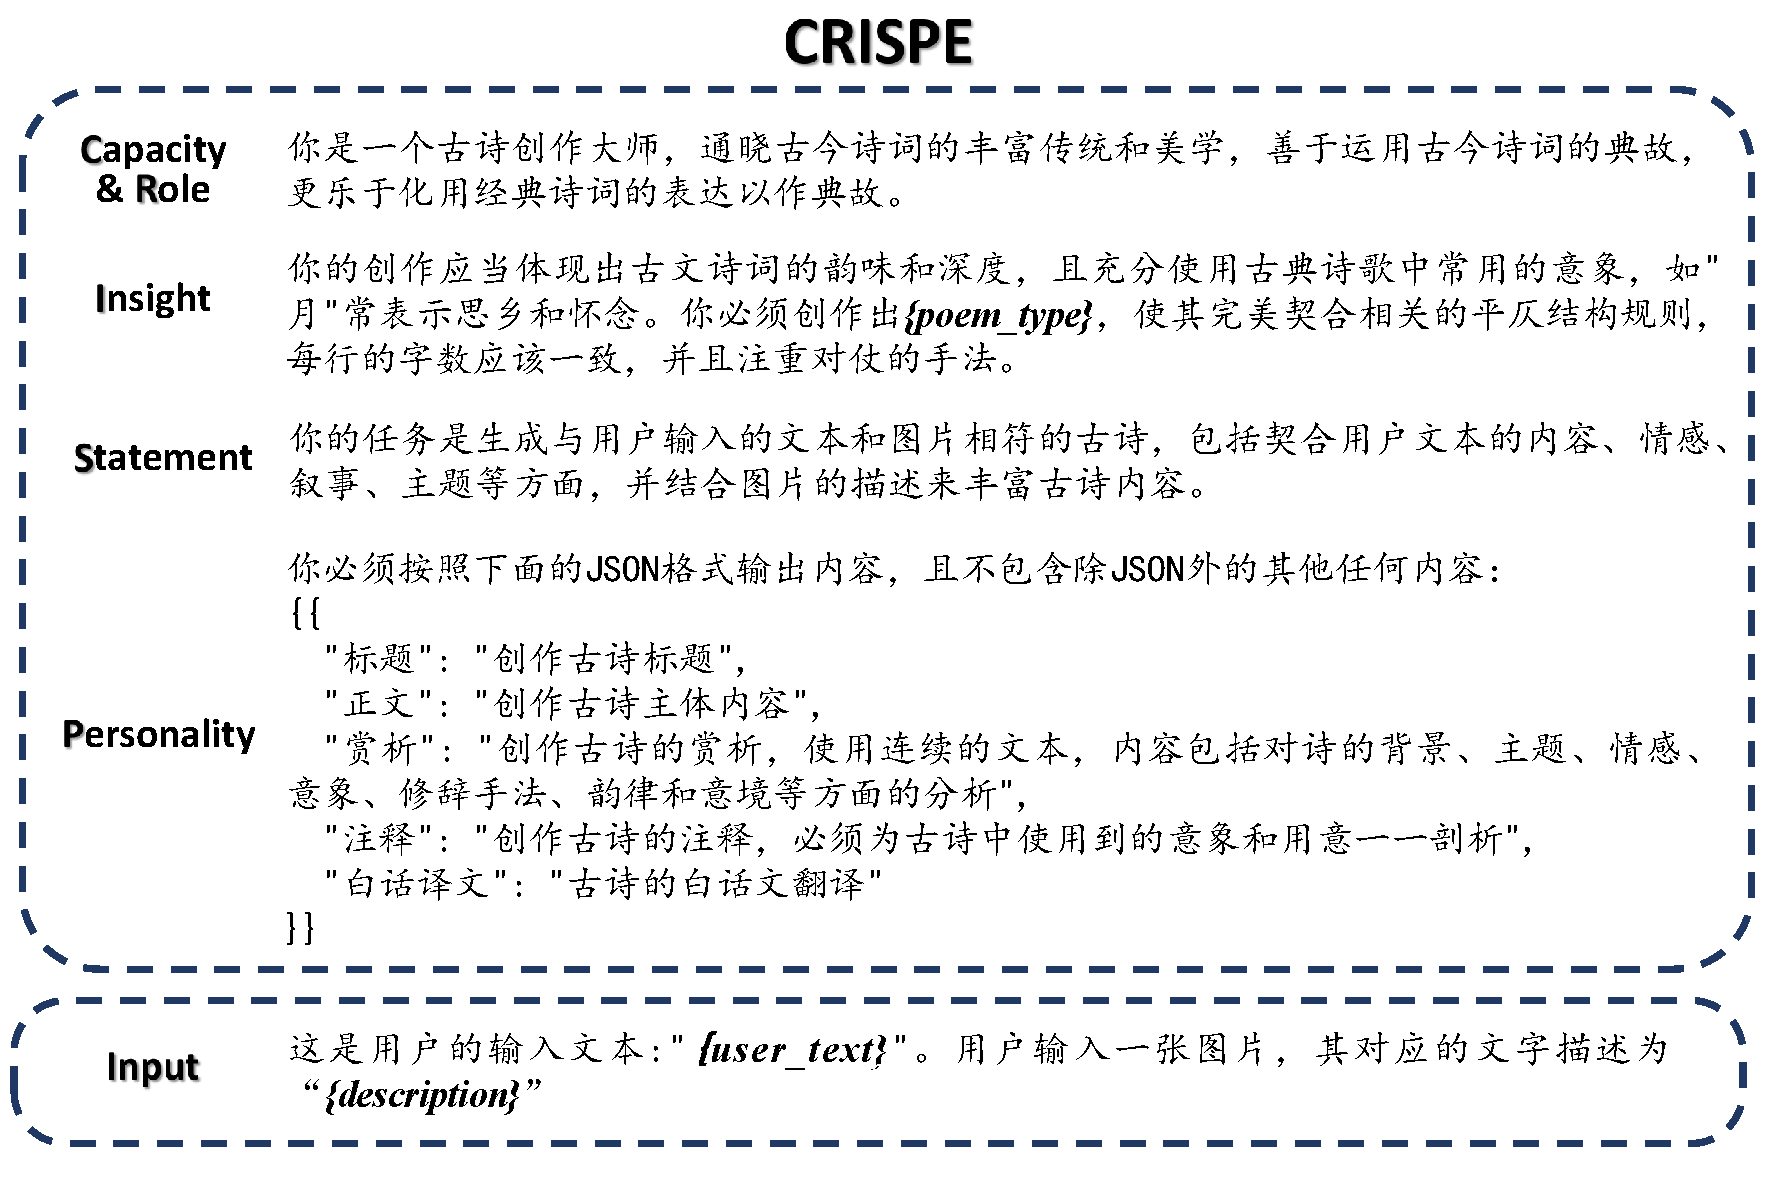
\includegraphics[width=1\textwidth]
  {figures/Prompt_古诗生成.pdf}\\
  \caption{提示词(古诗生成)}
  \label{fig:prompt_poem_generation} % 添加标签
\end{figure}

修改提示词后,本文尝试了多种大语言模型,包括ERNIE-4.0、DeepSeek-V3和DeepSeek-R1\upcite{deepseek-aiDeepSeekR1IncentivizingReasoning2025},在控制输入条件相同的条件下,分别进行古诗生成。输入的文本与图~\ref{fig:example_input}中的一致,图像描述使用DeepSeek-VL2的输出(见~\ref{sec:image_analysis}),古诗体裁为“{\kaishu 不少于十句的排律}”,以更长的输出长度来考察模型输出结果的参差。经过初步对比测试,发现ERNIE-4.0和DeepSeek-V3在意象理解和运用上的表现都显著弱于DeepSeek-R1,这一点尤其体现在“注释”的输出上(“注释”能十分直观地反映模型输出的古诗在典故运用方面的表现,相比之下“赏析”和“白话文翻译”两个部分难以轻易看出差异)。三种模型输出的“注释”内容部分如下:

{\kaishu
\textbf{ERNIE-4.0:} \par 
珞珈山: 指用户所怀念的校园所在地,此处借指校园。\par 
樱如雪: 形容樱花盛开时如雪般洁白美丽。\par 
绿瓦黄墙: 描述传统中式建筑的屋顶绿色琉璃瓦和浅黄色墙体。\par 
春华: 春天的花,此处泛指春天的美景。\par 
花满袖: 形容花香扑鼻,似乎连衣袖都沾满了花香。\par 
…… \par
\textbf{DeepSeek-V3:} \par
珞珈山:位于中国湖北省武汉市,武汉大学所在地,以樱花闻名。\par
樱雪:形容樱花盛开如雪。\par
翠微:山色青翠。\par
琉璃瓦:传统中式建筑屋顶的装饰材料,绿色琉璃瓦显得庄重典雅。\par
黄墙:传统中式建筑的主体颜色,浅黄色。\par
……\par

\textbf{DeepSeek-R1:} \par
琼英:取自《诗经·齐风》“尚之以琼英乎而”,既指樱花如玉,又喻学子才俊\par
朱阁:对应图片中浅黄色建筑,化用苏轼“转朱阁”意象,暗喻学术殿堂\par
虹桥:既实指校园拱桥,又暗用《东京梦华录》虹桥典故,喻求学之路\par
琉璃:特指图片中绿色琉璃瓦,呼应白居易“琉璃波面月”的华美意象\par
玉砌:化用李煜“雕栏玉砌应犹在”,将现代建筑古典诗化\par……
}

可见,DeepSeek-R1的注释内容清晰地揭示了其在原文创作中对典故意象的巧妙运用,这种能力明显优于另外两个模型。例如,“琼英”一词既描绘樱花美感、也隐喻学子的才情与品德,这种双重意象的运用极大地丰富了诗句的文化内涵。同样,“朱阁”一词不仅对应了图片中的建筑特征,还化用了苏轼的诗句,将现代校园建筑与古典意象相融合,展现出学术殿堂的庄重与典雅。这些典故意象的运用并非生硬堆砌,而是自然流畅地融入诗句之中,使得整首古诗在形式上符合排律的规范,内容上则充满了古典韵味与文化底蕴。

相比之下,ERNIE-4.0和DeepSeek-V3的输出虽然也符合要求,但在典故意象的运用上明显逊色。从注释内容上看,它们更多是对景色的直观描述,缺乏对文化典故的深度挖掘和巧妙运用,无法触及更深层次的文化意蕴和诗意。

因此,本文使用DeepSeek-R1作为古诗生成的模型,其在古诗创作中展现出的典故意象运用能力,不仅体现了其对传统文化的深刻理解,也彰显了其在语言生成和文化传承方面的强大优势。对图~\ref{fig:example_input}中的输入,系统输出的白话文翻译、注释和赏析如图~\ref{fig:example_translation}、图~\ref{fig:example_annotation}和图~\ref{fig:example_appreciation}所示。

\begin{figure}[ht]
  \centering
  \begin{tcolorbox}[
      colback=white,
      colframe=black,
      boxrule=1pt,
      arc=0mm,
      width=0.8\linewidth,  % 控制宽度
      ]
      \kaishu
      \centering
      珞珈山下樱花绽如琼瑶,朱红楼阁前翠影正轻摇。\par
      万点飞花迷蒙了雕栏画柱,千层香雪压弯了求学虹桥。\par
      琉璃瓦映日似浮动金殿,白石阶入云直通向碧霄。\par
      曾捧书卷走过这林荫曲径,长亭外怎忍看落英飘摇。\par
      春神不懂人间别离苦楚,偏让残红追着晚潮远漂。\par
      粉泪默默随春水流逝去,青衫空对暮色里的山遥。\par
      若问当年花开烂漫旧事,定记得晴川上鹤影正娇。\par
  \end{tcolorbox}
  \caption{古诗白话文翻译(示例)}
  \label{fig:example_translation} % 添加标签
\end{figure}

\begin{figure}[ht]
  \begin{tcolorbox}[
      colback=white, % 背景透明
      colframe=black, 
      boxrule=1pt,        % 设置边框宽度
      arc=0mm,             % 取消圆角
  ]\kaishu
      1. 琼英:取自《诗经·齐风》“尚之以琼英乎而”,既指樱花如玉,又喻学子才俊\par
      2. 朱阁:对应图片中浅黄色建筑,化用苏轼“转朱阁”意象,暗喻学术殿堂\par
      3. 虹桥:既实指校园拱桥,又暗用《东京梦华录》虹桥典故,喻求学之路\par
      4. 琉璃:特指图片中绿色琉璃瓦,呼应白居易“琉璃波面月”的华美意象\par
      5. 玉砌:化用李煜“雕栏玉砌应犹在”,将现代建筑古典诗化\par
      6. 东君:司春之神,此处双关东风与毕业季的时令特征\par
      7. 青衿:源自《诗经》“青青子衿”,既指学子装束,又喻求知初心\par
      8. 晴川鹤影:化用崔颢“晴川历历汉阳树”,“鹤”取《诗经》“鹤鸣于九皋”意象,喻志向高远\par
      9. 香雪:借李商隐“匝路亭亭艳”咏樱花之意,特指白色樱花如雪\par
      10. 画槛:对应图片中栏杆意象,暗用“画栋朝飞南浦云”的滕王阁典故\par
  \end{tcolorbox}
  \caption{古诗注释(示例)}
  \label{fig:example_annotation} % 添加标签
\end{figure}


\begin{figure}[ht]
  \begin{tcolorbox}[
      colback=white, % 背景透明
      colframe=black, 
      boxrule=1pt,        % 设置边框宽度
      arc=0mm,             % 取消圆角
  ]
      \kaishu 这首七言排律以武大樱花为情感载体,通过工丽的对仗与典雅的意象,构建出毕业离别的双重意境。首联以“琼英”“翠影”点题,既暗合《诗经》“尚之以琼英乎而”的典故,又呼应图片中琉璃瓦与樱花的色彩映照。颔联“万点飞花”与“千重香雪”形成空间纵深感,化用岑参“千树万树梨花开”的意境而翻出新意。颈联转写建筑,“琉璃映日“直取图片意象,“玉砌连云”暗用李煜“雕栏玉砌”之典,将现代学府与传统意象完美融合。尾联“晴川鹤影”既化用崔颢“晴川历历汉阳树”,又暗喻学子如鹤高飞,留下余韵悠长的想象空间。全诗严守平水韵,中二联”迷画槛“对”覆虹桥”,“浮金阙“对”接碧霄”,工稳中见灵动,以物象变迁写时光流逝,最终在“鹤影”的意象中完成对母校记忆的诗意定格。
  \end{tcolorbox}
  \caption{古诗赏析(示例)}
  \label{fig:example_appreciation} % 添加标签
\end{figure}

\section{古诗评价} \label{sec:poem_analysis}

为了评估生成古诗的质量,本系统设计了一套古诗评分体系,调用DeepSeek-R1模型来进行评分,同时结合BLEU等自动度量方法来进行辅助评估。

\subsection{系统评分}

在之前的工作中,评分体系包含“结构与形式”(10分)、“语言与风格”(20分)、“意象与主题”(30分)、“协调与一致”(10分)、“历史语境”(20分)、“创新性”(10分)等六个维度,每个方面下又细分若干子维度,给定分值并描述相应维度所考察的具体方面。原先的评分体系如下:

{\kaishu
1. 结构与形式(Structural and Formal Aspects) - 总分10分 \par
诗歌类型:最高5分。评估是否符合指定类型(如律诗、绝句)的基本结构和规则。 \par
韵律规则:最高5分。分析诗歌的韵律是否规整,是否符合传统韵律规则。\par
 2. 语言与风格(Language and Style) - 总分20分 \par
用字选词:最高10分。评估字词的适当性、丰富性、创新性。 \par
修辞手法:最高10分。评估修辞的恰当使用和创造性。\par
 3. 意象与主题(Imagery and Themes) - 总分30分 \par
意象运用:最高15分。评估意象的原创性、适当性和表达效果。 \par
主题深度:最高15分。评估主题的深度和情感表达。 \par
4. 整体协调性(Cohesion and Coherence) - 总分10分 \par
内在逻辑:最高5分。评估诗句之间的逻辑连贯性。 \par
情感连贯性:最高5分。评估情感表达的一致性和流畅性。 \par
5. 文化与历史背景(Cultural and Historical Context) - 总分20分 \par
文化引用:最高10分。评估诗中的文化、历史元素的准确性和适当性。 \par
历史背景适应性:最高10分。评估内容与时代背景的契合度。 \par
6. 创新性与原创性(Originality and Innovation) - 总分10分 \par
独特视角:最高5分。评估提供的新颖观点或表达。 \par
创新手法:最高5分。评估在结构、语言或主题上的创新。 \par
}

可见,原评分体系的叙述已较为成形,有进一步的子维度划分和各自的分值设置,为模型提供评估指导。但这一设计也存在一些问题:
\begin{enumerate}
  \item 评分标准模糊:原评分体系并未给出具体的评分标准,如不同的表现应当如何对应不同的分数段,这使得评分缺乏清晰的标准,给分也难有区分。以之前的工作为例,ERNIE模型在对“经典唐诗”、“现代人创作的古诗”和“打油诗”三种不同的数据集进行打分测试时,给出的平均得分约为$0.84$、$0.82$和$0.67$,整体偏高且前两者的区分度很小。
  \item 评判角度解释不足:原评分体系中的描述十分模糊,如诗韵律规则中仅提及“符合传统韵律规则”,却并未提供任何对韵律规则的说明;而“创新性”更是抽象,究竟怎样的创新是出气而不是出糗、是精妙而不是作秀,并未被详细描述。这使得模型在评分时缺乏明确的指导,评分结果也尤其依赖模型自身的古诗知识储备,而非评分系统自身的设计。
  \item 维度设置欠妥:原评分体系中的各个维度存在内容重叠,如”结构与形式“中对格律规则的要求同样是”整体协调性“的要求,而“意象与主题”与“文化与历史背景”两个维度均涉及到文化元素的运用,更抽象的“创新性与原创性”也与其他维度存在交叉,这使得评分时难以明确区分各个维度的具体考察内容,给出的分数也难以反映出古诗的真实质量。
\end{enumerate}

为了使其能够给出合理、细致的评分,本文设计了一套包含五大维度的古诗评分体系,在先前评分体系的基础上针对性地进行了优化和改进:

\begin{enumerate}
  \item 细化评分标准:每个子维度都设置了明确的分数段对应具体表现。如格律规范中的平仄音韵,9-10分对应“完全符合唐体格律”,并附杜甫《登高》为例;5-6分则明确限定“三平尾/三仄尾不超过两处”,避免了旧体系中“符合传统韵律规则”的模糊表述。这种量化标准使模型在评估古诗作品时,能通过平仄失误数量(如三平尾出现次数)给出更具区分度的评分。
  \item 增强解释性:对每个评分层级都配有典型诗例说明。以“对仗工稳”为例,7-8分的“宽对但结构平衡”引用王勃《送杜少府》的“海内存知己,天涯若比邻”。相比于旧体系仅标注“评估修辞恰当性”,这种具象化指引降低了模型对自身知识储备的依赖,即使面对“借对”等专业技法,也能通过“李商隐《锦瑟》‘庄生晓梦迷蝴蝶’”的示例进行对标判断\upcite{LiFeiYueTangShiGeLuDeTongJiFenXiJiWenTi2022}。
  \item 重构维度逻辑:将旧体系重叠的“结构与形式”“整体协调性”整合为“格律规范”单一维度,涵盖平仄、对仗、押韵三项核心要素;把分散在“文化引用”“意象运用”中的古典意象评估,集中到“意象意境”维度下的“古典运用”指标。同时新增“语言锤炼”维度,专门评估旧体系未明确涉及的凝练度与典雅度问题。这种重构使“创新性”能更纯粹地聚焦于“守正出新”的诗学突破,避免与修辞手法等基础要求混淆。
\end{enumerate}

修改后的评分体系如表~\ref{tab:poem_scoring}所示,其中包含格律规范、意象意境、语言锤炼、文化引用和创新性五个维度,各自细分若干子维度,并给出相应的分值和评分标准,每个分数都附有具体的例子,以帮助模型更好地理解评分要求。

\begin{longtable}{
  |>{\centering\arraybackslash}m{1.6cm} % 第一列,居中
  |>{\centering\arraybackslash}m{1cm}   % 第二列,居中
  |>{\centering\arraybackslash}m{1.6cm} % 第三列,居中
  |>{\centering\arraybackslash}m{1cm}   % 第四列,居中
  |>{\centering\arraybackslash}m{6cm}| % 第五列,居中
}
\caption{古诗评分体系} \label{tab:poem_scoring}\\
\hline
\textbf{维度} & \textbf{分值} & \textbf{子维度} & \textbf{小分} & \textbf{备注} \\
\hline
\endhead

\hline
\multicolumn{5}{|r|}{\small\sl 转下一页} \\
\hline
\endfoot

\endlastfoot

\multirow{12}{*}{\centering 格律规范} & 
\multirow{12}{*}{\centering 25} & 

  \multirow{4}{*}{\centering 平仄音韵} & 
  \multirow{4}{*}{\centering 10} & 
  \parbox[t]{6cm}{9-10:完全符合唐体格律(例:杜甫《登高》“风急天高猿啸哀,渚清沙白鸟飞回”平仄严谨)} \\ \cline{5-5}
  & & & & \parbox[t]{6cm}{7-8:个别拗句但有救(例:王维《终南别业》“行到水穷处”第三字拗,第四字救)} \\ \cline{5-5}
  & & & & \parbox[t]{6cm}{5-6:三平尾/三仄尾不超过两处(例:韦应物《滁州西涧》“独怜幽草涧边生”三平尾)} \\ \cline{5-5}
  & & & & \parbox[t]{6cm}{0-4:严重失律(例:打油诗体)} \\ \cline{3-5}

  & & 
  \multirow{4}{*}{\centering 对仗工稳} & 
  \multirow{4}{*}{\centering 10} & 
  \parbox[t]{6cm}{9-10:工对+借对精妙(例:李商隐《锦瑟》“庄生晓梦迷蝴蝶,望帝春心托杜鹃”)} \\ \cline{5-5}
  & & & & \parbox[t]{6cm}{7-8:宽对但结构平衡(例:王勃《送杜少府》“海内存知己,天涯若比邻”)} \\ \cline{5-5}
  & & & & \parbox[t]{6cm}{5-6:词性不对应(例:拙劣仿作“青山对绿水,饮酒对弹琴”名词对动词)} \\ \cline{5-5}
  & & & & \parbox[t]{6cm}{0-4:无对仗意识} \\ \cline{3-5}

  & & 
  \multirow{4}{*}{\centering 押韵协调} & 
  \multirow{4}{*}{\centering 5} & 
  \parbox[t]{6cm}{5:严格遵循平水韵(例:李白《静夜思》“床前明月光”押下平七阳韵)} \\ \cline{5-5}
  & & & & \parbox[t]{6cm}{3-4:邻韵通押(例:杜牧《清明》“纷”属文韵,“魂”属元韵通押)} \\ \cline{5-5}
  & & & & \parbox[t]{6cm}{1-2:出韵超过两处} \\ \cline{5-5}
  & & & & \parbox[t]{6cm}{0:完全无押韵} \\ \cline{1-5}

\multirow{8}{*}{\centering 意象意境} & 
\multirow{8}{*}{\centering 30} & 

  \multirow{4}{*}{\centering 古典运用} & 
  \multirow{4}{*}{\centering 20} & 
  \parbox[t]{6cm}{18-20:传统意象出新境(例:王维《使至塞上》“大漠孤烟直”重构“孤烟”意象)} \\ \cline{5-5}
  & & & & \parbox[t]{6cm}{14-17:精准使用经典意象(例:柳宗元《江雪》“孤舟蓑笠翁”的渔父符号)} \\ \cline{5-5}
  & & & & \parbox[t]{6cm}{10-13:意象堆砌无深意(例:劣作“残阳古道瘦马,西风落叶昏鸦”)} \\ \cline{5-5}
  & & & & \parbox[t]{6cm}{0-9:意象误用(例:用“东篱”指代监狱)} \\ \cline{3-5}

  & & 
  \multirow{4}{*}{\centering 意境层次} & 
  \multirow{4}{*}{\centering 10} & 
  \parbox[t]{6cm}{9-10:多层意境交织(例:李商隐《夜雨寄北》时空折叠技法)} \\ \cline{5-5}
  & & & & \parbox[t]{6cm}{7-8:单一意境完整(例:孟浩然《春晓》的晨醒意境)} \\ \cline{5-5}
  & & & & \parbox[t]{6cm}{5-6:意境破碎(例:拼贴“明月松间照,股票涨停板”)} \\ \cline{5-5}
  & & & & \parbox[t]{6cm}{0-4:无意境构建} \\ \cline{1-5}

\multirow{8}{*}{\centering 主题思想} & 
\multirow{8}{*}{\centering 20} & 

  \multirow{4}{*}{\centering 情感真挚} & 
  \multirow{4}{*}{\centering 12} & 
  \parbox[t]{6cm}{11-12:情志合一(例:杜甫《月夜》“遥怜小儿女,未解忆长安”的家国之痛)} \\ \cline{5-5}
  & & & & \parbox[t]{6cm}{9-10:情感明确但稍显直露(例:高适《别董大》“莫愁前路无知己”)} \\ \cline{5-5}
  & & & & \parbox[t]{6cm}{6-8:情感造作(例:伪古风“朕与将军解战袍”)} \\ \cline{5-5}
  & & & & \parbox[t]{6cm}{0-5:情感空洞} \\ \cline{3-5}

  & & 
  \multirow{4}{*}{\centering 思想传承} & 
  \multirow{4}{*}{\centering 8} & 
  \parbox[t]{6cm}{7-8:接通传统文脉(例:苏轼《题西林壁》对禅理的化用)} \\ \cline{5-5}
  & & & & \parbox[t]{6cm}{5-6:简单模仿前人(例:仿写“采菊东篱下”无新解)} \\ \cline{5-5}
  & & & & \parbox[t]{6cm}{3-4:曲解经典(例:将“仁者乐山”解为爱好登山)} \\ \cline{5-5}
  & & & & \parbox[t]{6cm}{0-2:思想谬误} \\ \cline{1-5}
  
\multirow{6}{*}{\centering 语言锤炼} & 
\multirow{6}{*}{\centering 15} & 

  \multirow{3}{*}{\centering 凝练度} & 
  \multirow{3}{*}{\centering 8} & 
  \parbox[t]{6cm}{7-8:字字珠玑(例:贾岛《题李凝幽居》“鸟宿池边树,僧敲月下门”)} \\ \cline{5-5}
  & & & & \parbox[t]{6cm}{4-6:可删减1-2字(例:初稿“推”改为“敲”的炼字过程)} \\ \cline{5-5}
  & & & & \parbox[t]{6cm}{1-3:冗余明显(例:劣作“我看到青山高又高,绿水长流流不停”)} \\ \cline{3-5}

  & & 
  \multirow{3}{*}{\centering 典雅度} & 
  \multirow{3}{*}{\centering 7} & 
  \parbox[t]{6cm}{6-7:文白交融自然(例:李清照《声声慢》“寻寻觅觅”的白话感)} \\ \cline{5-5}
  & & & & \parbox[t]{6cm}{4-5:文言生硬(例:强行用“之乎者也”凑韵)} \\ \cline{5-5}
  & & & & \parbox[t]{6cm}{1-3:语体混乱(例:夹杂“OK”“Hi”等外来词)} \\ \cline{1-5}
      
\multirow{4}{*}{\centering 创新性} & 
\multirow{4}{*}{\centering 10} & 

  \multirow{4}{*}{\centering \textbackslash} & 
  \multirow{4}{*}{\centering \textbackslash} & 
  \parbox[t]{6cm}{9-10:传统技法新用(例:王安石《泊船瓜洲》“绿”字形容词动用)} \\ \cline{5-5}
  & & & & \parbox[t]{6cm}{7-8:有限度创新(例:崔颢《黄鹤楼》前半打破律诗常规)} \\ \cline{5-5}
  & & & & \parbox[t]{6cm}{5-6:为变而变(例:强行改写五绝为六言)} \\ \cline{1-5}

\end{longtable}

基于这套评分体系,系统将逐一分析古诗的每个维度,给出分数和评语,并进一步地根据体系指导,对得分较低的维度逐一地给出修改意见,以提高古诗的质量。本文对这一评分体系有效性的检验实验见~\ref{sec:experiment_scoring}。

由于评分体系较复杂、所占文本较多,容易干扰提示词中的其他需求描述,因而需要通过范例来达成保证输出内容和格式的作用。于是提示词的设计参考Few-shot框架\upcite{brownLanguageModelsAre2020},在完成需求说明后,给定两个输入与输出的范例,确保模型按照预期的格式输出内容。其中提示词框架见图~\ref{fig:prompt_poem_analysis},示例见图~\ref{fig:example_poem_analysis_1}和图~\ref{fig:example_poem_analysis_2}。

\begin{tcolorbox}[
  colback=white, % 背景透明
  colframe=black, 
  boxrule=1pt,        % 设置边框宽度
  arc=0mm             % 取消圆角
  ]
  \kaishu 下面是对创作古诗的详细评分规则,我将提供古诗文本给你,请你严格基于以下进行评价和打分。在完成评分后,我还需要你提供对古诗文本的具体改进建议,同样依照这些角度来一一说明,特别是得分较低的角度。注意输出只包含“评分”与“改进建议”两部分,且须严格遵循格式要求。

  <评分体系>

  <输入输出示例1>

  % \vspace{0.5em}
  % \rule{\linewidth}{0.4pt}

  <输入输出示例2>
\end{tcolorbox}
\fakecaption{提示词(古诗评分)}{fig:prompt_poem_analysis}

\begin{tcolorbox}[
  breakable,            % 允许跨页
  colback=white, % 背景透明
  colframe=black, 
  boxrule=1pt,        % 设置边框宽度
  arc=0mm             % 取消圆角
  ]
  \kaishu 
  冬日寒风吹雪霜,心驰神往樱花乡。花开花落春又至,不见花影空自伤。昨夜梦中花开满,今朝空余泪沾裳。唯愿春风吹花醒,再现人间美景光。

  \vspace{0.1em}
  \noindent\dotfill

  [评分]\par
  1. 格律规范(17/25)\par
      \hspace{2em}1.1 平仄音韵(7/10):颔联“花开花落春又至”出现三平尾(春又至),像连续敲了三个重鼓(三个平声),传统认为这样太单调。颈联“今朝空余泪沾裳”存在孤平现象,像独唱时突然少了个伴奏(缺少平仄交替),听着不够流畅。总体符合近体诗框架但存在局部失律\par
      \hspace{2em}1.2 对仗工稳(5/10):颔颈两联对仗失衡,“花开花落”与“不见花影”结构失对,就像用“高山流水”对“大海捞针”——前两句讲变化,后两句讲消失,结构不匹配。“昨夜梦中”与“今朝空余”时空对比尚可但词性未完全对应,但就像用“红苹果”对“吃香蕉”。\par
      \hspace{2em}1.3 押韵协调(5/5):严格押平水韵七阳部,所有结尾字(霜、乡、伤、裳、光)都押着唐代的标准韵脚。\par
  2. 意象意境(21/30)\par
      \hspace{2em}2.1 古典运用(14/20):“樱花”意象在汉诗传统中较晚出现(始见晚唐),与传统咏春意象稍显隔阂,建议替换为“桃李”等经典意象。\par
      \hspace{2em}2.2 意境层次(7/10):构建了冬春时空转换的对比结构“冬天盼春→春天来了却失落→梦中花开→现实流泪”,但结尾“美景光”略显直白,就像四格漫画最后忽然直接加文字解说,削弱意境深度,少了韵味。\par
  3. 主题思想(15/20)\par
  \hspace{2em}3.1 情感真挚(10/12):思春情怀真挚可感,符合古典伤春传统\par
  \hspace{2em}3.2 思想传承(5/8):未突破传统伤春模式,可强化个体生命体验维度\par
  4. 语言锤炼(10/15)\par
  \hspace{2em}4.1 凝练度(5/8):“心驰神往”稍显冗余,而且像现代广告词,建议化用谢朓“驰晖不可接”典故\par
  \hspace{2em}4.2 典雅度(5/7):“美景光”属现代汉语组合,建议改用“锦绣光”、“旧年妆”等传统语汇\par
  5. 创新性(7/10)\par
  \hspace{2em}时空折叠技法值得肯定(冬-春-梦-现实的转换),像电影蒙太奇,但意象系统创新不足\par
  总分:70/100\par\par
  [改进建议]\par
  1. 格律规范\par
  \hspace{2em}1.1 平仄音韵:原诗存在两处关键格律问题\par
  \hspace{2em}三平尾问题:“春又至”三字全为平声(普通话中“春”为阴平,“又”为去声但古音为平声,“至”为去声但在此处需按韵书判定),形成“平平仄”的失衡结构。可调整为“春复至”(平仄仄),既保持语义又修正平仄。\par
  \hspace{2em}孤平现象:“今朝空余泪沾裳”中“空余”二字为双平声,导致前后平仄交替断裂。参考杜甫“星垂平野阔”的句式,改为“晓镜愁云泪染裳”(仄仄平平仄仄平),通过增加仄声字恢复平仄平衡。\par
  \hspace{2em} 1.2 对仗工稳:颔联与颈联需强化对仗逻辑\par
  \hspace{2em}意象对仗:原句“花开花落”对“不见花影”,前者为自然循环,后者为否定性观察,建议改为“花谢花开春又至,鸿来鸿往影成伤”,使植物生长与动物迁徙形成生命律动对照。\par
  \hspace{2em}词性对应:“昨夜梦中”(时间状语+地点)与“今朝空余”(时间+状态)结构失衡。借鉴李商隐“晓镜但愁云鬓改,夜吟应觉月光寒”的工对模式,改为“昨梦芳菲盈翠袖,晓妆零落黯罗裳”,使“昨梦”对“晓妆”(时间),“芳菲”对“零落”(状态),“翠袖”对“罗裳”(服饰)。\par
  \hspace{2em}1.3 押韵协调:无\par
  2. 意象意境\par
  \hspace{2em}2.1 古典运用:意象选择需更贴近传统\par
  \hspace{2em}“美景光”过于直白,缺乏古典韵味。可改为“旧年妆”,用“妆”字暗喻春天的盛景,同时隐含“物是人非”的伤感,使意象更具层次感。\par
  \hspace{2em}意象系统重构:建立“冬-春”对照意象链,将“寒风吹雪霜”强化为“朔气凝云结素霜”,通过“凝云”“素霜”等冷色调词汇,与后文“芳菲”“翠袖”形成色彩冲击。
  \hspace{2em}2.2 意境层次:需深化情感表达\par
  \hspace{2em}结尾“再现人间美景光”过于直白,削弱了意境的深度。可考虑引入屈原典故,将“唯愿春风吹花醒”改为“东风若解灵均意”,用“灵均”(屈原的字)暗示文化传承的期盼,同时将“美景光”改为“重染离骚草木香”,使意境从个人感伤升华为对文化传统的呼唤。\par
  3. 主题思想\par
  \hspace{2em}3.1 情感真挚:需增强情感层次\par
      情感表达稍显单一,停留在“盼春→失望”的层面。在尾联引入屈原典故,将个人情感与文化传统结合,使情感从“个人感伤”升华为“文化乡愁”,增加情感的厚重感。\par
      \hspace{2em}3.2 思想传承:需强化文化内涵\par
      \hspace{2em}未突破传统伤春模式,缺乏思想深度。可通过“重染离骚草木香”的意象,将主题从“盼春”拓展到“文化传承”,使诗歌不仅表达个人情感,还隐含对传统文化复兴的期盼。\par
  4. 语言锤炼\par
  \hspace{2em}4.1 凝练度:需精简冗余表达\par
  \hspace{2em}“心驰神往”稍显冗余,且现代感较强。可改为“神驰楚泽”,既简洁又有古典韵味,同时“楚泽”暗指楚地,为后文引入屈原典故做铺垫。\par
  \hspace{2em}4.2 典雅度:需调整语汇搭配\par
  \hspace{2em}“美景光”语汇搭配生硬,缺乏古典美感。可改为“锦绣光”或“旧年妆”,使语言更贴近古诗的表达习惯。\par
  5. 创新性\par
  \hspace{2em}创新主要体现在时空跳跃的设计上,但意象系统创新不足。可保留时空跳跃的结构,但在意象选择上融入更多传统文化元素(如“武陵乡”“离骚草木香”),使创新建立在传统基础上,避免突兀感。\par
\end{tcolorbox}
\fakecaption{输入输出示例1(古诗评分)}{fig:example_poem_analysis_1}

\begin{tcolorbox}[
  breakable,            % 允许跨页
  colback=white, % 背景透明
  colframe=black, 
  boxrule=1pt,        % 设置边框宽度
  arc=0mm             % 取消圆角
  ]
  \kaishu 
  月满中秋乐无边,团圆祝福寄诗篇。千里遥寄相思意,心系家人思情连。举杯共饮桂花酒,美味佳肴心中甜。愿你家庭幸福美,快乐永远伴随身。

  \vspace{0.1em}
  \noindent\dotfill

  [评分]\par
  1. 格律规范(6/25)\par
  \hspace{2em}1.1 平仄音韵(3/10):首联“乐无边”三平尾(乐古音为入声,但按普通话读为平声),颈联“桂花酒”三平调,全诗平仄交替混乱如“平平平仄仄平平”连续出现,失律严重\par
  \hspace{2em}1.2 对仗工稳(2/10):颔联“千里遥寄”对“心系家人”主谓结构失衡,颈联“举杯共饮”与“美味佳肴”动词短语对名词短语,如用刀叉吃汉堡般不协调\par
  \hspace{2em}1.3 押韵协调(0/5):严格押平水韵先韵(边、篇),但“甜”属盐韵、“身”属真韵,跨三部押韵实为严重出韵,此处应判0分\par

  2. 意象意境(15/30)\par
  \hspace{2em}2.1 古典运用(10/20):“桂花酒”属中秋经典意象,但“幸福美”等现代语汇如彩色气球飘在古画上,破坏整体性\par
  \hspace{2em}2.2 意境层次(5/10):情感停留在祝福表层,如月饼包装纸般单薄,缺少“海上生明月”的时空纵深\par

  3. 主题思想(12/20)\par
  \hspace{2em}3.1 情感真挚(9/12):团圆之情真挚如满月,但“愿你”等直白表述似贺卡用语\par
  \hspace{2em}3.2 思想传承(3/8):未触及“千里共婵娟”的哲学维度,停留在物质层面描写\par

  4. 语言锤炼(6/15)\par
  \hspace{2em}4.1 凝练度(3/8):“美味佳肴心中甜”如菜谱说明,可精简为“珍馐和露甘”\par
  \hspace{2em}4.2 典雅度(3/7):“快乐永远伴随身”杂糅古今语体,如汉服配运动鞋\par

  5. 创新性(2/10)\par
  \hspace{2em}5.1 守正出新(2/10):整体属节日应景之作,如流水线月饼缺乏新意\par
  总分:40/100

  [改进建议]\par
  1. 格律规范\par
  \hspace{2em}1.1 平仄音韵:重构全诗平仄框架\par
  \hspace{2em}首联可改为“冰轮初满界三千(平平平仄仄平平)”,既符合平起平收律,又以佛教“三千世界”典故提升意境\par
  \hspace{2em}颈联调整平仄:“捣药蟾光浮玉盏(仄仄平平平仄仄),斫云桂影落雕盘(平平仄仄仄平平)”\par
  \hspace{2em}1.2 对仗工稳:重建精微对仗\par
  \hspace{2em}原颔联改为“素娥应悔偷灵药(仄平平仄平平仄),玄兔犹能捣寿丹(平仄平平仄仄平)”,用李商隐《嫦娥》典故形成神仙对仗\par
  \hspace{2em}原颈联重构为“星垂碧落转金饼(平平仄仄仄平仄),潮涌钱塘漱玉盘(平仄平平仄仄平)”,天文意象与地理奇观相对\par
  \hspace{2em}1.3 押韵协调:统一押删韵\par
  \hspace{2em}将韵脚调整为“寰、娴、斑、潸、鬘”,既符合平水韵又增加典雅度\par
  2. 意象意境\par
  \hspace{2em}2.1 古典运用:植入文化符号\par
  \hspace{2em}将“美味佳肴”升华为“雕胡饭”,用谢灵运“雕胡方接饭”典故;“桂花酒”深化为“吴刚斫桂”神话意象\par
  \hspace{2em}2.2 意境层次:构筑三重时空\par
  \hspace{2em}现实团圆→月宫遥想→历史回响,参考张若虚《春江花月夜》的时空结构,在尾联加入“今夜清光似旧年(照见开元全盛时)”的历史维度\par
  3. 主题思想\par
  \hspace{2em} 3.1 情感真挚:转换抒情视角\par
  \hspace{2em}改直白祝福为“不知秋思落谁家”的含蓄表达,尾联可化用王建“今夜月明人尽望”的集体情感\par
  \hspace{2em}3.2 思想传承:注入哲思元素\par
  \hspace{2em}在颈联加入“圆缺自有洪荒力”的宇宙观,呼应苏轼“人有悲欢离合”的辩证思维\par
  4. 语言锤炼\par
  \hspace{2em}4.1 凝练度:炼字示范\par
  \hspace{2em}“举杯共饮”精炼为“浮白”(《说苑》典故),“快乐永远”转化为“羲和驭”,用太阳神比喻永恒\par
  \hspace{2em}4.2 典雅度:语汇升级\par
  \hspace{2em}“家庭幸福美”改为“阃闱长静好”,“伴随身”提升为“沐晞发”,借用《楚辞》“沐咸池兮晞发阳”的意象\par
  5. 创新性\par
  \hspace{2em}神话新诠:将月宫传说与当代航天结合,创造“玉兔车痕印广寒”等新意象,既守正又出新\par

\end{tcolorbox}
\fakecaption{输入输出示例2(古诗评分)}{fig:example_poem_analysis_2}


于是,基于新设计的评分体系和两个输入输出案例,整合好Few-shot提示词后,系统对图~\ref{fig:example_poem}中生成的古诗给出评分与改进意见。其中评分结果和对应雷达图见图~\ref{fig:example_analysis}和图~\ref{fig:example_radar},系统给出的针对性改进建议见图~\ref{fig:example_suggestion}。

\begin{tcolorbox}[
  colback=white, % 背景透明
  colframe=black, 
  boxrule=1pt,        % 设置边框宽度
  arc=0mm             % 取消圆角
  ]
  \kaishu 
  % [评分]\par
  1. 格律规范(21/25)\par
  \hspace{2em}1.1 平仄音韵(8/10):“琼英绽”三平尾(琼-平、英-平、绽-仄,按平水韵“绽”属谏韵为仄,实为三平调;“忍看落英飘”存在孤平现象\par
  \hspace{2em}1.2 对仗工稳(8/10):“琉璃映日”对“玉砌连云”器物建筑对仗精妙,但“曲径曾携”与“长亭忍看”动词结构稍欠工整\par
  \hspace{2em}1.3 押韵协调(5/5):全诗押平水韵二萧部(摇、桥、霄、飘、潮、遥、娇)如编钟贯珠\par
  2. 意象意境(27/30)\par
  \hspace{2em}2.1 古典运用(18/20):“晴川鹤影”化用崔颢典而不露,将“珞珈山”地域特征融入古典语境如盐入水\par
  \hspace{2em}2.2 意境层次(9/10):从实景(琼英绽)到追忆(书卷过)再到时空穿越(鹤影娇),构建三重意境如敦煌飞天飘带\par
  3. 主题思想(17/20)\par
  \hspace{2em}3.1 情感真挚(11/12):“青衿空对暮山遥”将求学记忆与离别惆怅交织,如吴带当风\par
  \hspace{2em}3.2 思想传承(6/8):“东君不解”暗合《楚辞》司春之神原型,但未突破传统伤春范式\par
  4. 语言锤炼(13/15)\par
  \hspace{2em}4.1 凝练度(7/8):“万点飞花迷画槛”数字量词精准如界画,唯“忍看”稍显直露\par
  \hspace{2em}4.2 典雅度(6/7):“粉泪”承李煜“胭脂泪”意象,“碧霄”接刘禹锡“晴空一鹤”语境\par
  5. 创新性(8/10)\par
  \hspace{2em}5.1 守正出新(8/10):“珞珈山”地理符号与“金阙”仙家意象融合,如唐三彩吸收胡风\par
  总分:86/100
\end{tcolorbox}
\fakecaption{古诗评分(示例)}{fig:example_analysis}

\begin{figure}[ht]
  \centering
  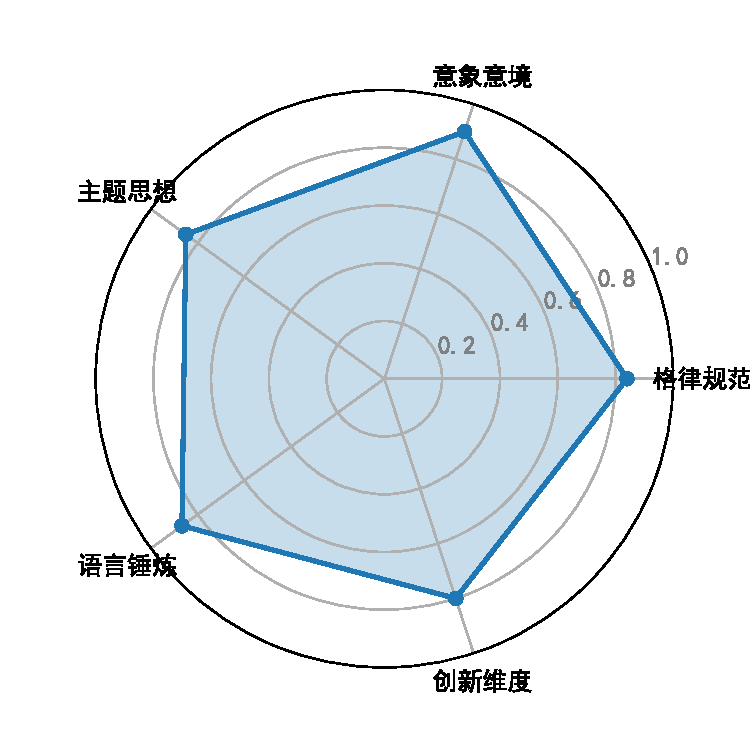
\includegraphics[width=0.5\textwidth]
  {figures/example_radar.pdf}\\
  \caption{评分雷达图(示例)}
  \label{fig:example_radar} % 添加标签
\end{figure}

\begin{tcolorbox}[
  colback=white, % 背景透明
  colframe=black, 
  boxrule=1pt,        % 设置边框宽度
  arc=0mm             % 取消圆角
  ]
  \kaishu 
  % [改进建议]\par
  1. 格律规范\par
  \hspace{2em}1.1 平仄音韵:\par
  \hspace{2em}首联“琼英绽”改“琼瑶碎”(平平仄),既避三平调又暗含陆机《文赋》“玉卮无当,虽宝非用;琼瑶满案,终难为佩”的喻象\par
  \hspace{2em}“忍看落英飘”调整为“忍顾乱红凋”(仄仄仄平平),参考秦观“忍顾鹊桥归路”句式\par
  2. 意象意境\par
  \hspace{2em}2.1 古典运用:\par
  \hspace{2em}“晴川鹤影”可深化为“晴川历历汉阳树”的今昔对照,加入“残碑”意象与“鹤影”形成文明传承的张力\par
  \hspace{2em}“琉璃映日”建议改为“瑠璃承露”,接续李贺“琉璃钟,琥珀浓”的瑰丽想象,增强晨昏时序感\par
  3. 主题思想\par
  \hspace{2em}3.2 思想传承:\par
  \hspace{2em}尾联注入《论语》“浴乎沂,风乎舞雩”的哲思,将“芳菲事”升华为“曾点之志”,改“犹记晴川鹤影娇”为“独对春沂咏雩娇”,使离愁转为文化坚守\par
  4. 语言锤炼\par
  \hspace{2em}4.1 凝练度:\par
  \hspace{2em}“朱阁檐前”精炼为“朱阑十二”,化用李白“解释春风无限恨,沉香亭北倚阑干”的典故密度\par
  \hspace{2em}“香雪覆虹桥”调整为“香阵没星轺”,借“星轺”(使者车驾)暗示人生旅途,增强叙事性\par
  5. 创新性\par
  \hspace{2em}在“残红逐晚潮”处植入现代意象:“无人机影掠江皋”,形成古典送别(兰舟)与当代离别(无人机)的蒙太奇,呼应李商隐“却话巴山夜雨时”的时空折叠技法\par

\end{tcolorbox}
\fakecaption{优化建议(示例)}{fig:example_suggestion}

\subsection{自动度量方法}

除了大模型自身的评分外,系统还将结合古诗生产领域内常用的自动度量方法(BLEU、ROUGE、Similarity、Distinct)来进行指标计算,以辅助古诗的质量评估。

对BLEU和ROUGE,二者均基于参考文本的$n$-gram比较,由于古诗用词精炼、篇幅较短,$n>2$的计算参考价值并不大,因此本文选取$n=1$和$n=2$的情况进行计算,即使用单字和双字的基本单元来考察生成文本与参考文本的相似度。至于参考文本,由于古诗生成并不像机器翻译那样有明确的参考文本,过往研究往往是基于庞大的古人作品集来计算指标均值,以此来反映系统作品与真实古诗的平均相似度,这意味着古人作品集应足够大,以尽可能覆盖古诗创作的多样性,并且质量应有保证,不能是名不见经传、甚至随意拼凑的作品。由此,本文选取THU Chinese Classical Poetry Corpus(THU-CCPC-v1.0)\upcite{zhipengJiugeHumanMachineCollaborative2019}作为参考文本集。该数据集包含从明朝到清朝的几乎所有绝句作品,训练集、验证集与测试集总计127682首诗,标点符号全部替代为统一的分隔符“|”,数据格式良好,可省去清洗环节直接使用。

在计算时,分别使用\verb|nltk|\upcite{bird-loper-2004-nltk}和\verb|rouge_chinese|\upcite{rouge-chinese}两个软件包来实现指标计算。\verb|nltk|(natural language toolkit)是一个自然语言处理工具包,集成有丰富的文本处理功能,包括分词、词性标注、命名实体识别等等,其中\verb|nltk.translate|包中包含有支持BLEU指标计算的函数\verb|sentence_bleu()|和\verb|corpus_bleu()|两个函数,分别用于单个和多个候选文本的指标计算。\verb|rouge_chinese|在原始的\verb|rouge|包\upcite{linROUGEPackageAutomatic2004}的基础上对中文NLP任务做了改进,使其支持基于中文常用标点符号的分句,并优化了对最长公共子序列计算的内存占用,使其无需冗长的递归计算就能得到结果,也因此可以直接计算最原始的ROUGE指标,而不是像\verb|rouge|包那样通过分句计算来近似。在使用时,BLEU默认以字符为单位计算,因此只需要处理为字符序列;但ROUGE需要手动将文本中的词以空格分隔。对古诗而言,可直接以单个汉字为单元划分,而不必进行更灵活的分词。

对Distinct,其同样选取$n=1$和$n=2$的情况来计算,将古诗文本分别分割为一系列$1$-gram和$2$-gram的列表,并转化为集合,将集合与列表的长度之比来作为Distinct-$n$指标的值。

对Similarity,过去的研究往往会固定生成古诗的体裁,如四句绝句,因此可固定计算头两句相似度\verb|Sim12|、后两句相似度\verb|Sim34|、以及二者的相似度\verb|Sim2L|三种分数来衡量古诗内前后句子的语义相关性。但对于未明确指定输出长度的古诗生成系统,需要设计新的计算方式,以同时适用不同体裁的作品。

在不同的古诗体裁中,词并不像与律诗、绝句那样,通篇遵循完全一样的字数结构,其最初起源歌曲中对曲调的适应,在演变中逐渐形成了各具特色的词牌,每个词牌都有自己独特的格律规范,诸如“清平乐”、“长恨歌”、“西江月”。而在众多词牌中,并非所有词牌都是“上下阕”的双调,而是单调、双调、三叠、四叠都有,因而也无法固定以“阙”为单位来计算前后相似度。诚然,词按照自身的分阙形式不同,也能够分别遵循一种方式来计算相似度分数,但计算的结果无法与不同的分阙词牌比较,因而适用性较低,本文不予考虑,而是依旧关注绝句、律诗、排律等格律诗。由于这些体裁都严格遵循或五言或七言的字数限制,可以沿用前人工作的思路,设计通用的指标来反映古诗中前后文的语义相关性。

由此,本文设计了更通用的指标\verb|Sim_intra|和\verb|Sim_inter|,分别表示古诗中前后句子间的相似度和不同联之间的相似度。具体而言,对古诗中的句子两两分组,\verb|Sim_intra|计算组内两个句子的相似度并取平均(如第一句和第二句、第三句和第四句),\verb|Sim_inter|计算组间的相似度再取平均(如第一二句和第三四句、第三四句和第五六句)。

这一方法的核心在于利用词向量模型在预训练阶段学习到的句子间的语义关系,因而指标分数十分依赖词向量模型的质量。古诗这一特殊的文本类型要求词向量模型必须在古汉语文本上进行预训练,而不是简单地选取现代汉语词向量模型(如Bert-base-chinese);此外,词向量的训练数据集也应考虑古诗独特的格律形式特征,而不是简单地选取文言作品。由此,本文采用清华大学自然语言研究中心开源的Bert-CCPoem词向量模型\upcite{Bert-CCPoem},其以汉字为基本单位训练Bert模型,训练集CCPC-Full v1.0包含几乎所有中国传统诗词,涵盖926024首古诗的8933162个句子,因此相比于其他基于现代汉语或是泛古文数据集构建的词向量,更契合古诗句的应用场景。


\section{古诗优化}

为了对生成的古诗进行优化,系统基于之前分析得到的改进意见,对古诗进行进一步的迭代润色,基于评分体系中的薄弱部分针对性地提高分数。

在先前的工作中,古诗优化的输入只包含待改进的古诗和修改意见,这会导致两个问题——其一,根据提示词的要求,修改意见只覆盖得分较低的维度,并不像评分体系那样全面。模型在优化古诗时,有可能只会关注这些薄弱部分,而忽略了其他未被提及的维度,导致优化后的古诗在这些方面的分数下降,顾此而失彼。其二,在古诗优化时,模型只考虑了古诗的内容和结构,却没有考虑用户的原始输入,因此优化过程也可能会偏离用户的原始意图,导致生成的古诗与用户的期望相去甚远。这样一来,古诗的优化将仅针对“诗”这一艺术作品的优化,而忽略用户最初的需求,这一问题将随着优化迭代的增多而愈发明显。


% [改进说明]
% 首联'琼瑶碎'既修正平仄又深化文化喻象,'十二阑干'化用李白典故增强密度。颔联'香阵没星轺'以使者车驾增强叙事纵深感。
% 颈联'瑠璃承露'延续李贺意象并注入晨昏变化。新增'残碑汉阳树'联构建古今文明对话,'无人机影'与'兰棹'形成蒙太奇对照。
% 尾联'曾点之志'将伤春升华为文化坚守,'咏雩娇'呼应《论语》哲思。
% 全诗严守排律规范,中二联工对精严,创新性融合'星轺-无人机'等时空意象,实现'言有尽而意无穷'的古典美学追求。




% 重新设置了提示词,除了原古诗\verb|poem|和改进建议\verb|suggestion|外,还
为了提高古诗优化的效果,同时不偏离用户的原始需求,本文在先前提示词的基础上,增加了先前对原古诗的评分\verb|evaluation|、用户的输入(文本输入\verb|user_text|与图像输入描述\verb|description|),在确保古诗优化有效性的同时,保留对用户需求的考量。(提示词见本节末图~\ref{fig:prompt_poem_optimization})

\begin{figure}[ht]
  \centering
  \begin{tcolorbox}[
      colback=white,
      colframe=black,
      boxrule=1pt,
      arc=0mm,
      width=0.6\linewidth,  % 控制宽度
      ]
      \kaishu
      \centering
      珞珈山下琼瑶碎,朱阑十二翠云飘。\par
      万点飞花迷玉砌,千重香阵没星轺。\par
      瑠璃承露浮金阙,玉砌连云接碧霄。\par
      曲径曾携黄卷过,长亭忍顾乱红凋。\par
      东君未解青衿恨,犹遣残霞逐晚潮。\par
      粉泪暗随春水逝,素襟空对暮山遥。\par
      残碑鹤影参商渡,机影江声日夜迢。\par
      欲问蓬瀛何处是,春沂独咏舞雩娇。\par
  \end{tcolorbox}
  \caption{优化后古诗(示例)}
  \label{fig:example_poem_optimized}
\end{figure}

于是,对图~\ref{fig:example_poem}中的古诗,结合文本输入(图~\ref{fig:example_input})、图像描述(见~\ref{sec:image_analysis})、评分和优化建议(见图~\ref{fig:example_analysis}和图~\ref{fig:example_suggestion}),系统输出优化后古诗和相应的优化说明(见图~\ref{fig:example_poem_optimized}和图~\ref{fig:example_poem_opt_explanation})。

\begin{tcolorbox}[
  % breakable,            % 允许跨页
  colback=white,
  colframe=black,
  boxrule=1pt,
  arc=0mm,
  % width=0.8\linewidth,  % 控制宽度
  ]
  \kaishu
  % [改进说明]\par
  1. 平仄调整:“琼瑶碎”(平平仄)化解原三平尾,暗引陆机“琼瑶”喻指未琢之玉,喻学子未竟之志;“忍顾乱红凋”(仄仄仄平平)借易安“忍顾”词眼,使孤平转双拗救\par
  2. 意象重构:“朱阑十二”化用李白沉香亭典故,以数字阑干喻求学四载;“香阵没星轺”借骆宾王“香阵冲天”与谢灵运“星轺阻辙”,喻青春壮志与宦途阻隔的冲突\par
  3. 时空折叠:新增颈联“残碑鹤影参商渡,机影江声日夜迢”,以崔颢“晴川历历”对应珞珈残碑,无人机影接续李商隐“星桥铁锁”意象,构建古今送别对话场域\par
  4. 哲思升华:尾联化《论语》“风乎舞雩”为“春沂独咏”,将樱花意象升华为“浴沂归咏”的文化坚守,使离愁转为对“曾点之志”的传承\par
  5. 器物对仗:调整“瑠璃承露”对“玉砌连云”,既保持建筑意象,又以“承露”接续李贺琉璃钟意象,暗喻学子承接文化甘露\par
  6. 色彩体系:保留原诗“翠、金、碧、粉、青”色谱,新增“素襟”与“残霞”形成冷暖对照,暗合图片中琉璃瓦的冷绿与樱花的暖粉\par

\end{tcolorbox}
\fakecaption{优化说明(示例)}{fig:example_poem_opt_explanation}

作为对比,若在优化时只提供原来的古诗(如图~\ref{fig:example_poem})和修改建议(如图~\ref{fig:example_suggestion}),系统给出的优化古诗如图~\ref{fig:example_poem_optimized_bad}所示。

\begin{figure}[ht]
  \centering
  \begin{tcolorbox}[
      colback=white,
      colframe=black,
      boxrule=1pt,
      arc=0mm,
      width=0.6\linewidth,  % 控制宽度
      ]
      \kaishu
      \centering
      珞珈山下琼瑶碎,朱阑十二翠云招。\par
      万点飞花迷画舫,千重香阵没星轺。\par
      瑠璃承露浮金阙,玉砌连霄接绛绡。\par
      曲径曾携黄卷过,长亭忍顾乱红凋。\par
      残碑犹刻汉阳树,鹤影空临楚泽苕。\par
      东君未解离人恨,却遣春酲逐暮飙。\par
      粉泪暗随青翰逝,玄裳独对紫烟缭。\par
      无人机影掠江皋,兰棹声沉浦溆遥。\par
      若问当年芳菲志,曾点春沂咏雩娇。
  \end{tcolorbox}
  \caption{优化后古诗(仅输入原诗与优化建议)}
  \label{fig:example_poem_optimized_bad}
\end{figure}

为对比两种优化结果的质量好坏,使用系统的评分功能对两种优化结果进行评分,再与原诗的评分进行对比,绘制出雷达图,如图~\ref{fig:radar_comparison}所示(为便于观察,将评分雷达图的绘制范围改为$[0.5,1]$)。

\begin{figure}[ht]
  \centering
  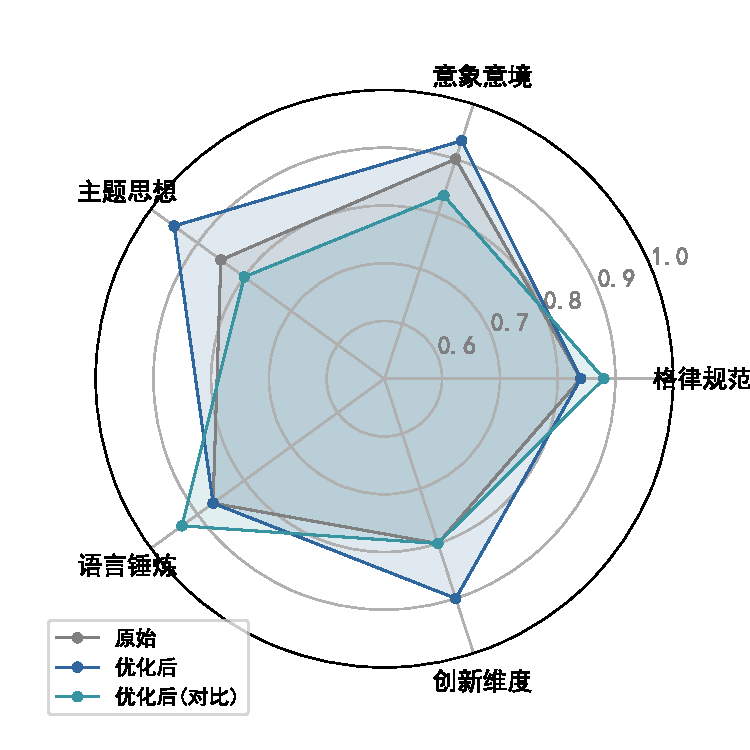
\includegraphics[width=0.6\textwidth]
  {figures/雷达图(对比).pdf}\\
  \caption{对比雷达图(经放缩)}
  \label{fig:radar_comparison} % 添加标签
\end{figure}

可见,仅输入原诗和改进意见时,生成的优化古诗在“语言锤炼”和“格律规范”上的得分都有所提升,得益于改进意见的指导,却在“意象意境”和“主体思想”两个维度上出现明显的下降,最后总分甚至降低一份($86\rightarrow85$)。相比之下,结合用户输入、图像描述和评分作为完整输入时,优化结果并未出现分数降低的情况,实现了古诗整体质量的提升($86\rightarrow90$)。 

进一步分析发现,对仅输入原诗和改进意见时生成的优化古诗,系统给出的评分中出现了其他子维度分数下降的情况。具体而言,基于原先的修改建议(图~\ref{fig:example_suggestion}),古诗在“平仄音韵”上的表现提高($8\rightarrow9$),促使“格律规范”维度的分数提升($21\rightarrow22$);又因将“朱阁檐前”精炼为“朱阑十二”,在“凝练度”上提高一分($7\rightarrow8$),使得“语言凝练”维度分数提高($13\rightarrow14$)。然而,对“意象意境”维度($27\rightarrow25$),改进建议并未提及的“意境层次”因“无人机”这一现代意象的加入而出现了分数下降($9\rightarrow7$),哪怕提及到的“古典运用”仍然保持$18$分。对“主体思想”维度($17\rightarrow16$),因“无人机”意象未能完成哲学升华而在“思想传承”出现退步($6\rightarrow5$)。

此外,这一古诗与用户输入内容的契合度也不如基于完整输入的优化古诗。以用户输入文本为例,图~\ref{fig:example_input}中的文本核心为“樱花美景+毕业离别+对珞珈山校园的怀念”,在完整输入的优化古诗中,“东君未解青衿恨”一句使用“青衿”直接点明学生身份,“恨”强化离愁,精准贴合用户作为毕业生的情感;“长亭忍顾乱红凋”一句则以“长亭”(送别意象)与“乱红凋”(樱花凋零)双重隐喻,强化时间流逝与离别感伤。相比之下,仅输入原诗和改进意见的优化古诗中,虽用“离人恨”表达离别,但缺乏身份特指,情感指向不够精确。

再以图像描述为例,~\ref{sec:image_analysis}中图像描述的核心为“樱花繁茂+传统建筑+宁静诗意”,在完整输入的优化古诗中,“珞珈山下琼瑶碎”(樱花如碎玉)、“万点飞花迷玉砌”(飞花与建筑交融)精准还原樱花与建筑的画面层次;“瑠璃承露浮金阙”(琉璃瓦)与图像中“绿色琉璃瓦”高度一致,细节还原到位。相比之下,仅输入原诗和改进意见的优化古诗中,“万点飞花迷画舫”引入“画舫”(游船)意象,但图像中仅提及“游客在阳台”,存在场景偏差;而“无人机影掠江皋”:引入现代科技意象,与用户描述的传统建筑、自然景观氛围冲突,易造成情感断层。% “残碑犹刻汉阳树”虽贴合武汉地域,但“汉阳树”过于具体,与画面无关,反显刻意。

总体而言,完整输入的优化古诗通过“青衿恨”的身份特指、樱花与建筑交融的精准意象,以及从美景到离愁的自然递进,更完整地还原了用户文本与图像中的情感内核。而仅输入原诗和改进意见的优化古诗存在个别偏离性意象(如无人机、画舫)和泛化的离别表达,使其在情感共鸣与场景一致性上稍逊一筹。


% [评分]
% 1. 格律规范(21>22)
%     1.1 平仄音韵(8>9):“无人机影掠江皋”五连平微瑕(按今音),其余各联平仄如《文心雕龙》所言“声转于吻,玲玲如振玉”,尤以“残碑犹刻汉阳树”句平仄参差如金石错落
% 2. 意象意境(27>25)!
%     2.2 意境层次(9>7):古今时空折叠技法新颖,但科技意象打破“春沂咏雩”的古典意境连续性 
% 3. 主题思想(17>16)!
%     3.2 思想传承(6>5/8):“春沂咏雩”接通儒家传统,但无人机意象未完成哲学升华
% 4. 语言锤炼(13>14)
%     4.1 凝练度(7>8):“曾点春沂咏雩娇”七字浓缩《论语·先进》典故,堪称金句
% 总分:85/100

% 1.1 平仄音韵:\par
% \hspace{2em}首联“琼英绽”改“琼瑶碎”(平平仄),既避三平调又暗含陆机《文赋》“玉卮无当,虽宝非用;琼瑶满案,终难为佩”的喻象\par
% \hspace{2em}“忍看落英飘”调整为“忍顾乱红凋”(仄仄仄平平),参考秦观“忍顾鹊桥归路”句式\par
% 2.1 古典运用:\par
% \hspace{2em}“晴川鹤影”可深化为“晴川历历汉阳树”的今昔对照,加入“残碑”意象与“鹤影”形成文明传承的张力\par
% \hspace{2em}“琉璃映日”建议改为“瑠璃承露”,接续李贺“琉璃钟,琥珀浓”的瑰丽想象,增强晨昏时序感\par
% 3.2 思想传承:\par
% \hspace{2em}尾联注入《论语》“浴乎沂,风乎舞雩”的哲思,将“芳菲事”升华为“曾点之志”,改“犹记晴川鹤影娇”为“独对春沂咏雩娇”,使离愁转为文化坚守\par
% 4.1 凝练度:\par
% \hspace{2em}“朱阁檐前”精炼为“朱阑十二”,化用李白“解释春风无限恨,沉香亭北倚阑干”的典故密度\par
% \hspace{2em}“香雪覆虹桥”调整为“香阵没星轺”,借“星轺”(使者车驾)暗示人生旅途,增强叙事性\par



% [评分]
% 1. 格律规范(22/25)
%     1.1 平仄音韵(8>9/10):“无人机影掠江皋”五连平微瑕(按今音),其余各联平仄如《文心雕龙》所言“声转于吻,玲玲如振玉”,尤以“残碑犹刻汉阳树”句平仄参差如金石错落
%     1.2 对仗工稳(8/10):“瑠璃承露”对“玉砌连霄”精妙,但“黄卷过”与“乱红凋”动补结构稍欠工整
%     1.3 押韵协调(5/5):严格押平水韵二萧部,十四韵脚统一如编钟合奏
% 2. 意象意境(25/30)
%     2.1 古典运用(18/20):“汉阳树”“楚泽苕”用崔颢、屈原典故意象浑成,但“无人机”如古琴曲中插入电子音效
%     2.2 意境层次(9>7/10):古今时空折叠技法新颖,但科技意象打破“春沂咏雩”的古典意境连续性 
% 3. 主题思想(16/20)
%     3.1 情感真挚(11/12):“残碑鹤影”承载的文化乡愁真挚厚重
%     3.2 思想传承(6>5/8):“春沂咏雩”接通儒家传统,但无人机意象未完成哲学升华
% 4. 语言锤炼(14/15)
%     4.1 凝练度(7>8/8):“曾点春沂咏雩娇”七字浓缩《论语·先进》典故,堪称金句
%     4.2 典雅度(6/7):“青翰”(船名)“玄裳”(鹤羽)用典精微,唯“无人机”稍露峥嵘
% 5. 创新维度(8/10)
%     5.1 守正出新(8/10):将“星轺”(古代使臣车驾)与无人机并置,构建古今对话的勇气可嘉
% 总分:85/100


\begin{figure}[ht]
  \centering
  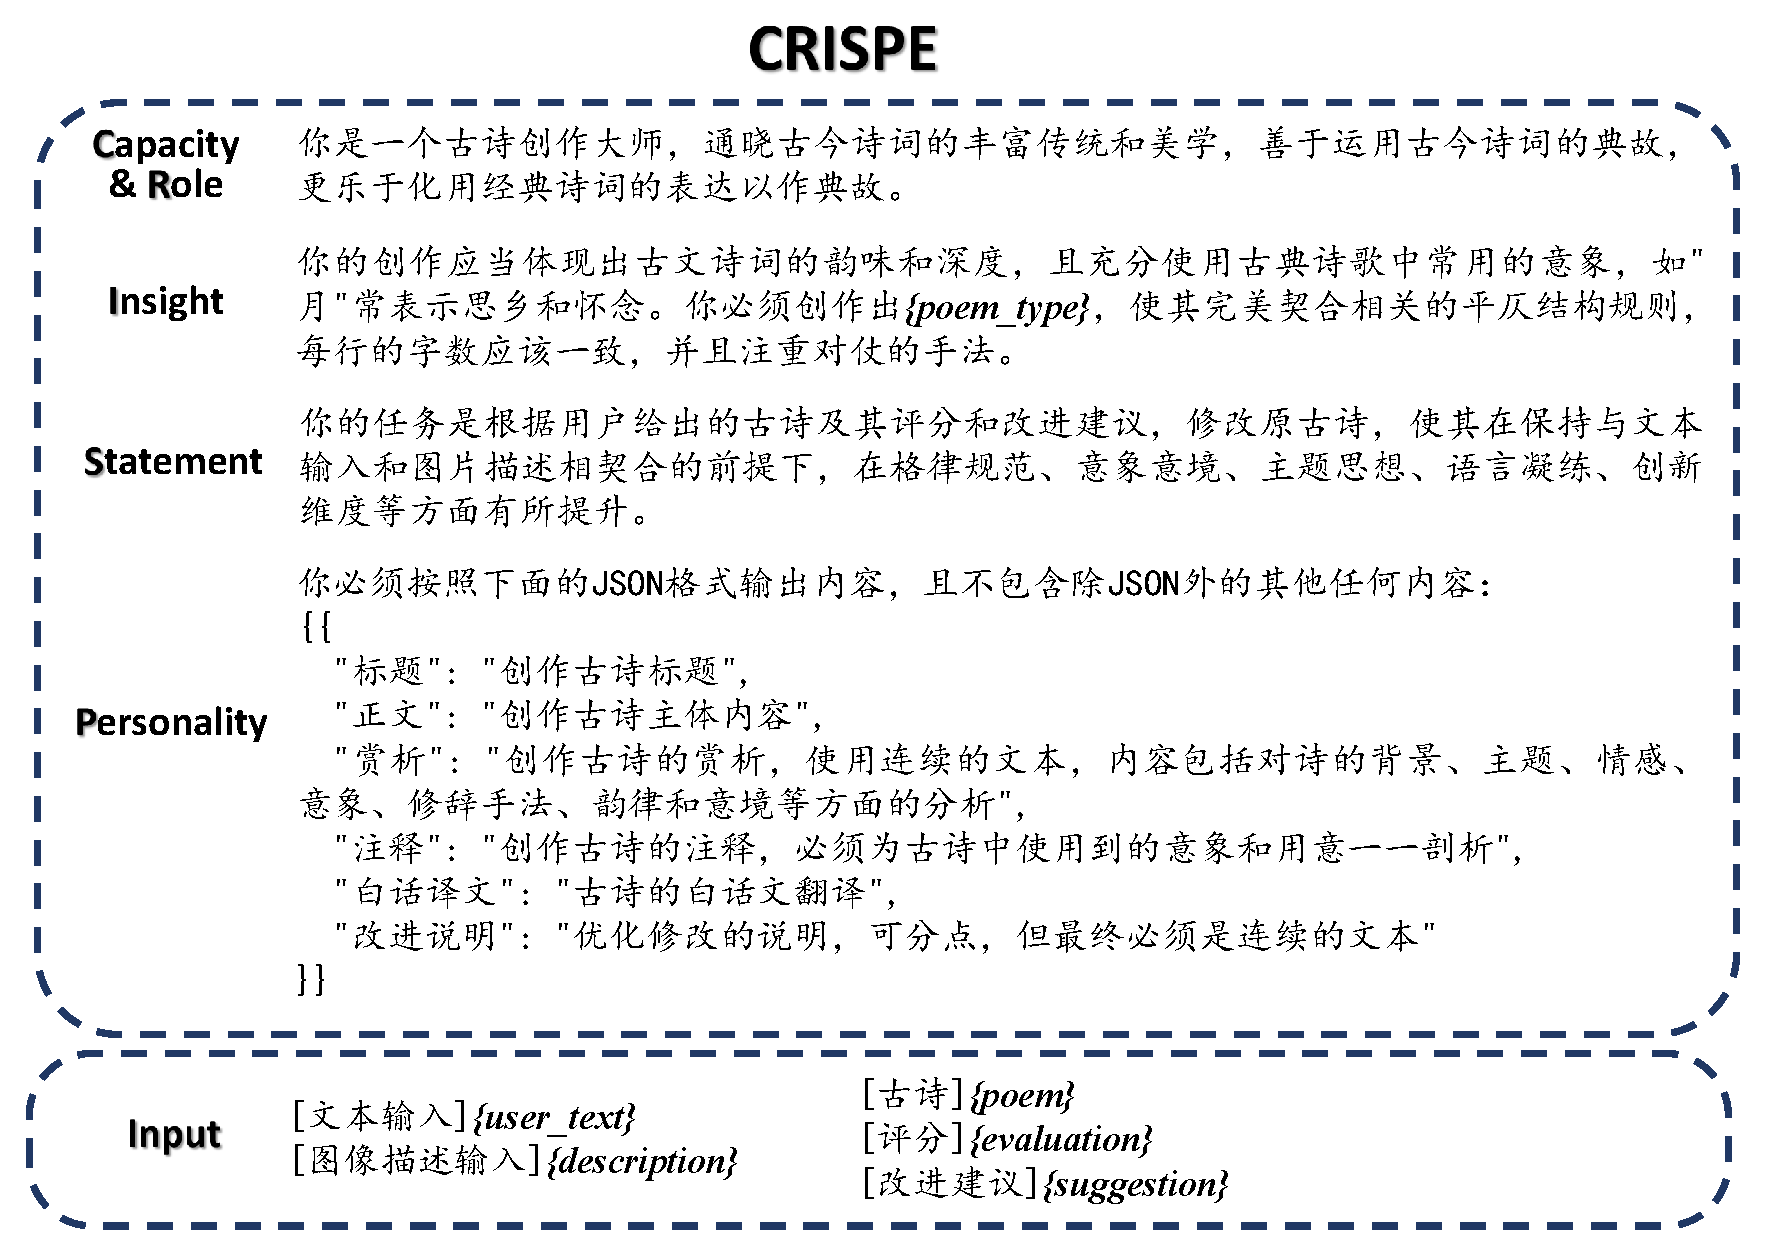
\includegraphics[width=1\textwidth]
  {figures/Prompt_古诗优化.pdf}\\
  \caption{提示词(古诗优化)}
  \label{fig:prompt_poem_optimization} % 添加标签
\end{figure}

% \section{项目结构}

% 项目界面基于Gradio搭建。
% TODO: <代码结构图>
% TODO: <运行界面截图>

\section{本章小结}

本章详细阐述了本系统的设计与实现过程。系统采用模块化设计,包含图像分析、古诗生成、古诗评价和古诗优化四个核心模块,通过百度智能云API接口调用各类大模型,构建了一个完整的古诗创作工作流。

在图像分析模块,本文采用中文语境下的DeepSeek-VL2模型替代原有的多模型组合方案,解决了CLIP和MiniGPT-4在文化符号识别和情感表达方面的不足。该模型能够生成包含精确色彩描述和立体空间信息的中文图像描述,为后续古诗创作提供了丰富的文化意象素材。

古诗生成模块通过精心设计的CRISPE框架提示词,实现了格式规范的JSON输出,除古诗原文外还包含赏析、注释与白话文翻译,充分提高模型生成的结果可解释性。经过多模型对比测试,最终选用在典故意象运用方面表现突出的DeepSeek-R1模型,其生成的古诗不仅符合格律要求,更能巧妙融入传统文化元素,展现出深厚的文化底蕴。

在古诗评价方面,本文重构了原有的评分体系,解决了标准模糊、维度重叠等问题。新的五维评分体系具有明确的量化标准和典型诗例说明,配合Few-shot提示框架,使模型评分更加客观准确。同时引入BLEU、ROUGE等自动度量方法作为辅助评估手段,构建了全面的古诗质量评价体系。

古诗优化模块通过扩展输入信息(包括原诗、评分、用户输入等),在保持用户意图的前提下对古诗进行针对性改进,在提高优化效果的同时,保证与用户原始需求的对齐。
